\section{Circuit components and orthogonal fields}\label{sec:fields}

The finite identity in this section is independent of the geometry of a
triangulation.  Geometry enters only when we assign displacement vectors to
its sides.  A component beside a dual circuit, rather than the whole side of
that circuit, is the coordinate of the identity. We first obtain the
separate second-moment identities for the two displacement fields and
then use stationarity to control their complete macroscopic rim sums.

\subsection{An exact identity on a triangulated sphere}

Fix a finite simple triangulation $T$ of the oriented sphere, and give its
vertices independent fair colors.  Draw its trivalent dual $\Gamma$ through
the interiors of the triangles.  A dual edge is \emph{occupied} when the
endpoints of the primal edge it crosses have different colors.  At a dual
vertex there are either zero or two occupied edges.  The occupied subgraph
is therefore a union of vertex-disjoint simple circuits.

In fact its law is uniform on the even subgraphs of $\Gamma$.  To see this,
prescribe a set of primal edges across which the spin changes.  Spins can be
recovered, starting from one vertex, precisely when the number of prescribed
changes around every primal cycle is even.  The face boundaries generate the
cycle space of a spherical triangulation, so it is enough to check the
triangular faces.  These are exactly the even-degree conditions in the dual.
Every allowable prescription has the two spin assignments obtained from one
another by interchanging the colors.

For each occupied circuit $L$, take the connected components $C$ of the
topological graph $\Gamma\setminus L$: all points of $L$, including its
vertices, are removed.  In particular, an open edge whose two endpoints have
been removed can be a component by itself.  Figure~\ref{fig:component-labels}
illustrates the deletion convention in the tetrahedral dual.
Put $\lambda=(L,C)$ and, for a
point $m$ in the interior of a dual edge, define
\[
 H_\lambda(m)=\ind_{\{m\in C\}}.
\]
Vectors indexed by these pairs, with the index set taken separately in each
configuration, have the scalar product
\[
 \langle F,G\rangle
   =\Esp\sum_\lambda F_\lambda\overline{G_\lambda}.
\]
Here and throughout the finite discussion, $\Esp$ averages colors with the
triangulation fixed.  Write $H(m)=(H_\lambda(m))_\lambda$ and
$K(m,n)=\langle H(m),H(n)\rangle$.

\begin{figure}[tbp]
\centering
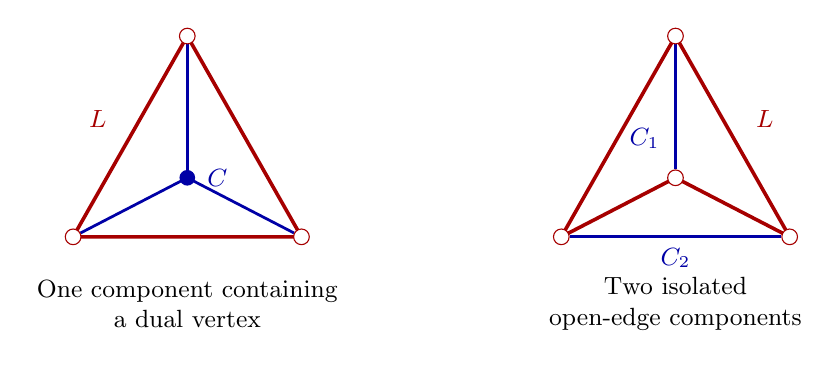
\begin{tikzpicture}[
  wall/.style={red!65!black,line width=1.3pt},
  component/.style={blue!65!black,line width=1pt,shorten <=3pt,shorten >=3pt},
  deleted/.style={circle,draw=red!65!black,fill=white,inner sep=2pt},
  retained/.style={circle,fill=blue!65!black,inner sep=2pt},
  every node/.style={font=\small}]
\begin{scope}[xshift=-3.1cm]
  \coordinate (a) at (0,1.55);
  \coordinate (b) at (-1.45,-1);
  \coordinate (c) at (1.45,-1);
  \coordinate (d) at (0,-.25);
  \draw[wall] (a)--(b)--(c)--cycle;
  \draw[component,shorten >=0pt] (a)--(d);
  \draw[component,shorten >=0pt] (b)--(d);
  \draw[component,shorten >=0pt] (c)--(d);
  \foreach \v in {a,b,c} \node[deleted] at (\v) {};
  \node[retained] at (d) {};
  \node[blue!65!black,right] at (.13,-.25) {$C$};
  \node[red!65!black,left] at (-.9,.5) {$L$};
  \node[align=center] at (0,-1.85)
    {One component containing\\a dual vertex};
\end{scope}
\begin{scope}[xshift=3.1cm]
  \coordinate (a) at (0,1.55);
  \coordinate (b) at (-1.45,-1);
  \coordinate (c) at (1.45,-1);
  \coordinate (d) at (0,-.25);
  \draw[wall] (a)--(b)--(d)--(c)--cycle;
  \draw[component] (a)--(d);
  \draw[component] (b)--(c);
  \foreach \v in {a,b,c,d} \node[deleted] at (\v) {};
  \node[blue!65!black,left] at (-.08,.25) {$C_1$};
  \node[blue!65!black,below] at (0,-1.02) {$C_2$};
  \node[red!65!black,right] at (.9,.5) {$L$};
  \node[align=center] at (0,-1.85)
    {Two isolated\\open-edge components};
\end{scope}
\end{tikzpicture}
\caption{Components in the tetrahedral dual $\Gamma=K_4$.
The heavy red circuit $L$ and its hollow vertices are shown for reference
but are deleted. The remaining blue graph has one component in the left
panel and two in the right panel; its endpoints at deleted vertices are excluded.
Components are determined by connectivity in $\Gamma\setminus L$.}
\label{fig:component-labels}
\end{figure}

\begin{lemma}[Two defects]\label{fields:defects}
For distinct edge-interior points $m,n$, subdivide the dual edges at these
points and take a uniform subgraph with odd degree at $m,n$ and even degree
elsewhere.  Then $K(m,n)$ is the expected number of circuits in this
subgraph.  The assertion also applies to distinct points on the same edge.
\end{lemma}

\begin{proof}
For any even set $D$ of vertices of a connected finite graph, the subgraphs
with boundary $D$, when nonempty, form an affine translate of the cycle
space.  Toggling a path between two prescribed defects gives such a
translation.  In particular, the even and two-defect ensembles have the same
cardinality; subdividing an edge does not change that cardinality.

In the present two-defect ensemble, ordinary vertices have occupied degree
zero or two, while the degree-two marked vertices have occupied degree one.
Thus there is one simple defect path and a collection of disjoint circuits.
Fix a possible circuit $L$.  When it is occupied, every third edge at a
vertex of $L$ is unoccupied.  A defect path must consequently lie in
$\Gamma\setminus L$.  The circuit can occur in the defect ensemble only if
$m,n$ lie in the same component of this complement.  If they do, fix a path
between them in that component.  Toggling it bijects even subgraphs
containing $L$ with two-defect subgraphs containing $L$.  Hence
\[
 \PP_{m,n}(L\text{ occupied})
 =\PP_{\varnothing}(L\text{ occupied})
   \ind_{\{m,n\text{ in one component of }\Gamma\setminus L\}}.
\]
Summing over $L$ proves the assertion.  If the two marks lie on one edge,
its open interior connects them whenever that edge is not in $L$, even when
both endpoints of the edge belong to $L$.
\end{proof}

At a dual vertex corresponding to a triangle $t$, choose points
$m_j(t)$ on its three spokes, indexed by $j=0,1,2$ in positive cyclic order.
Choose the star neighborhoods disjoint.  With
$\om=\exp(2\pi\ii/3)$, set
\[
 Z_t=\sum_{j=0}^2\om^jH(m_j(t)).
\]

\begin{proposition}[Finite orthogonality]\label{fields:orthogonality-prop}
For distinct triangles $t,u$,
\begin{equation}\label{fields:orthogonal}
 \langle Z_t,Z_u\rangle=0,
 \qquad \|Z_t\|^2=\frac34.
\end{equation}
\end{proposition}

\begin{proof}
For the off-diagonal identity, start with uniform oddness at the two dual
vertices $t,u$.  Toggle the short segment from $t$ to $m_j(t)$ and that from
$u$ to $m_k(u)$.  This moves the defects to the two marked points and
preserves uniformity.  By \cref{fields:defects}, it suffices to take the
$\sum_{j,k}\om^{j-k}$ Fourier sum of the resulting circuit counts.

Delete the interiors of the two small stars.  For a fixed initial
configuration, what remains consists of circuits and paths pairing its
occupied star ports.  Each star has either one or three such ports.  The
outside circuits contribute a constant.  If a star has one occupied port,
the modified defect path uses that port regardless of which short segment
was toggled, so the circuit count is independent of that star's index.
These terms vanish in the Fourier sum.

It remains to consider three occupied ports at each star.  There are two
possibilities.  With one through path, the two other ports at each star are
paired by an outside cap.  If $r_t,r_u$ are the through ports, the additional
circuit count after moving the defects is
\[
 \ind_{\{j=r_t\}}+\ind_{\{k=r_u\}}.
\]
It is a sum of one-index terms and again has zero double Fourier sum.  With
three through paths, let $\pi$ be their matching of ports.  An additional
circuit is formed exactly when $k=\pi(j)$: the other two through paths then
join into one circuit.  Disjoint paths between the two boundary circles of
the punctured sphere reverse their positive cyclic orders, so
$\pi(j)=\ell-j\pmod 3$ for some $\ell$.  Their contribution is
\[
 \sum_{j=0}^2\om^{j-\pi(j)}
   =\om^{-\ell}\sum_{j=0}^2\om^{2j}=0.
\]
This establishes the cancellation for each initial configuration, including
when $t,u$ are adjacent.

For the norm, a circuit avoiding $t$ places the three nearby spoke points in
one component, whose Fourier sum is zero.  If $t$ is occupied, exactly one
circuit passes through it.  The two used spokes belong to that circuit,
while the missing spoke belongs to exactly one complementary component.
Thus $Z_t$ has precisely one nonzero coordinate, of modulus one, in this
case.  The three distinct primal vertices of $t$ are not all the same color
with probability $3/4$, proving the second identity.  Equivalently, any
diagonal kernel in this calculation can be evaluated using two distinct
points of the same spoke, which have identical $H$-vectors; coincident
defects are never needed.
\end{proof}

\subsection{The two displacement fields}

Suppose $t$ is drawn as a straight triangle in an oriented plane chart.
Let $z_t$ be its barycenter, and let $d_{tj}$ be the complex side vector
dual to spoke $j$, traversed clockwise around $t$.  Since the three side
vectors sum to zero, there are unique $p_t,q_t\in\C$ such that
\begin{equation}\label{fields:side-decomposition}
 d_{tj}=p_t\om^j+q_t\overline{\om}^{j},
 \qquad
 p_t=\frac13\sum_jd_{tj}\om^{-j},
 \quad q_t=\frac13\sum_jd_{tj}\om^j.
\end{equation}
Applying the real affine map from an equilateral triangle to $t$ gives
\begin{equation}\label{fields:area}
 |p_t|^2-|q_t|^2=\frac4{\sqrt3}\Area(t),
 \qquad |p_t|+|q_t|\le C\diam(t).
\end{equation}
Indeed the two Fourier coefficients are the complex-linear and
antilinear parts of this map, whose Jacobian is their squared-modulus
difference; the equilateral case fixes the constant and sign.

A triangle $t$ is \emph{tagged} for $\lambda=(L,C)$ by $j$ if $L$ uses $t$
and its missing spoke $j$ belongs to $C$.  For a coefficient function $g$
supported where the side vectors are defined, put
\begin{align*}
 U_\lambda(g)&=\sum_{t\text{ tagged by }j}g(z_t)p_t\om^j,\\
 Q_\lambda(g)&=\sum_{t\text{ tagged by }j}g(z_t)q_t\overline{\om}^{j},
 &V_\lambda(g)&=U_\lambda(g)+Q_\lambda(g).
\end{align*}
Changing the first spoke index changes the Fourier coefficients by the
inverse phases, so the summands are well defined.  A rotation of the chart
multiplies each of the two summands by the corresponding complex rotation.

The $\lambda$-coordinate of $Z_t$ is exactly $\om^j$ when $t$ has that tag,
and is zero otherwise.  Its conjugate gives the other phase.  Consequently
\cref{fields:orthogonal} gives the exact identities
\begin{equation}\label{fields:energy}
 \Esp\sum_\lambda |Q_\lambda(g)|^2
   =\frac34\sum_t|g(z_t)q_t|^2,
 \qquad
 \Esp\sum_\lambda |U_\lambda(g)|^2
   =\frac34\sum_t|g(z_t)p_t|^2.
\end{equation}
In particular,
\begin{equation}\label{fields:V-energy}
 \Esp\sum_\lambda |V_\lambda(g)|^2
 \le \frac32\sum_t|g(z_t)|^2\bigl(|p_t|^2+|q_t|^2\bigr).
\end{equation}
We call these the \emph{Bessel bounds}.  The coefficients may be arbitrary
complex numbers depending on the graph and its geometry, but must be
independent of its colors.  Continuity is not required.  In particular,
these bounds apply to deterministic spatial masks.  The sums include every
component, including isolated open edges.

\subsection{Rims and their extremality}

\begin{lemma}[Component rims]\label{lemma:rim}
If $C$ contains a dual vertex, the union of the closed primal triangles
whose centers belong to $C$ has one simple monochromatic boundary circuit
$P$.  Orient $P$ with $C$ on its left.  Its right-hand triangles are exactly
the tags of $(L,C)$, one per edge, and their facing third vertices belong to
one cluster of the opposite color.  The oriented circuit $P$ determines
$(L,C)$.

If $C$ contains no dual vertex, it is an isolated open edge.  It has exactly
two tags.  When they are in one plane chart, their contributions satisfy
\begin{equation}\label{fields:isolated}
 V_{(L,C)}(g)=\bigl(g(z_t)-g(z_u)\bigr)d_{te},
 \qquad V_{(L,C)}(1)=0,
\end{equation}
where $t,u$ are its endpoint triangles and $e$ their common missing side.
\end{lemma}

\begin{proof}
The triangles with centers in $C$ are connected through shared sides.
A boundary side separates such a triangle from a triangle visited by $L$;
the latter's missing spoke leads into $C$.  This identifies the boundary
sides with the tags.

At a primal vertex, the sectors belonging to $C$ form one cyclic interval,
unless they fill its entire neighborhood.  Otherwise choose two separated
runs of $C$-sectors.  Each intervening interval contains an $L$-sector: an
immediately adjacent untouched triangle would still connect to $C$.
Extend two selected $C$-sectors and two intervening $L$-sectors to alternating
points of a sufficiently small circle about the primal vertex, using short
segments inside the sectors.  Outside that circle they are joined in the
two disjoint connected sets $C$ and $L$.  Two disjoint connected sets in
the complementary disk cannot join alternating boundary contacts, a
contradiction.

It follows that the union of the closed $C$-triangles is a connected
subsurface of the sphere with disjoint simple boundary circuits.  Each
boundary circuit faces a different complementary disk.  The connected
circuit $L$ avoids this subsurface and faces it across every boundary side,
so there can be only one such disk and one boundary circuit.  This is $P$.
The missing side at an occupied triangle has equal-colored endpoints;
hence all vertices of $P$ have the same color.  Following either side of a
disagreement circuit gives a connected walk of constant color: within a
visited triangle the adjacent site either stays the same or changes across
an edge joining two sites of that color.  The vertices facing $P$ therefore
lie in one opposing cluster.

Any directed edge of $P$ identifies its occupied right triangle and thus
$L$; its left triangle identifies $C$.  Finally, a component with no dual
vertex must be one open edge with both endpoints on $L$.  Those endpoints
give its two tags, whose side vectors are opposite.  This proves
\eqref{fields:isolated}.  Their separate $U$- and $Q$-contributions need not
vanish.
\end{proof}

We call $P$ an oriented \emph{rim} and write $U_P,Q_P,V_P$ for the
corresponding fields.  If its entire drawing is in plane coordinates,
$V_P(1)$ is the sum of its oriented edge displacements, and hence is zero.
Restricting \eqref{fields:energy} to genuine rims gives inequalities; the
equalities themselves retain the isolated components.

\begin{lemma}[No right bypass and its converse]\label{lemma:no-bypass}
A rim has no path of its own color joining two distinct rim vertices with
all its other points in the open right-hand disk.  Conversely, a simple
monochromatic circuit with this property, and with an opposite-colored site
in its right-hand disk, is a rim.
\end{lemma}

\begin{proof}
An alleged bypass may be made simple.  It is a crosscut of the right-hand
disk and separates its two nonempty rim arcs.  Choose an edge on each arc.
Its facing triangle lies on that arc's side of the crosscut, since a
primal graph path cannot cross the interior of a face.  Its opposing
vertex does not lie on the bypass.  Thus the two facing vertices are in
different parts of the cut disk.  Their opposing cluster can cross neither
the monochromatic rim nor the monochromatic bypass, contradicting
\cref{lemma:rim}.

For the converse, let $uv$ be an edge of the given circuit and $w$ the third
vertex of its right triangle.  If $w$ had the circuit color and lay strictly
on the right, $u,w,v$ would be a bypass.  If $w$ belonged to the circuit,
one of $uw,wv$ would be a right-side chord, unless the right disk were that
single triangular face.  The latter possibility has no opposite-colored
site and is excluded by hypothesis.  Every facing vertex is therefore of
the opposite color.

Choose the occupied dual circuit $L$ through one facing triangle.  It
cannot cross the monochromatic circuit, so it stays on its right.  The
triangles on the left are untouched and form part of one component $C$
off $L$.  Its rim $P^*$ includes the chosen edge and lies in the closed
right side of the original circuit, since its left subsurface contains
the original left disk.  If the two circuits differed, a segment of $P^*$
between successive contacts with the original circuit would be a right
bypass.  Such a segment has distinct endpoints by simplicity: follow
$P^*$ from the common edge to its first departure and then to its next
contact.  This contradicts the hypothesis, proving equality.
\end{proof}

\begin{lemma}[Sandwich]\label{lemma:sandwich}
In an annular band, suppose that there are disjoint essential simple black
and white circuits, with the white circuit on the right of the black one
for the direction of the band.  There is a black rim, with this direction,
in the closed region between them.
\end{lemma}

\begin{proof}
Take a maximal biconnected block of the black graph containing the given
black circuit.  The face of this block toward the white circuit has a
simple boundary.  That boundary lies between the two given circuits:
the block contains the black one and cannot cross the white one.  A black
bypass in this face would add an ear between two distinct vertices of the
block and enlarge the block, contrary to maximality.  The white circuit
supplies an opposite-colored site in the face.  Apply
\cref{lemma:no-bypass}.  In the full plane the same argument uses the finite
black cluster containing the given circuit.
\end{proof}

\subsection{Infinite volume and closed sums}

The local estimates of \cref{sec:probability} imply the following facts
for Poisson--Voronoi percolation.  There are almost surely no infinite
monochromatic clusters: the one-arm bound tends to zero as the outer
radius tends to infinity, and a countable collection of inner boxes covers
the plane.  An infinite disagreement wall would have infinite connected
site chains on both its sides, so every occupied wall is finite as well.

The dual graph has one end.  Indeed, enclose any finite removed part and
all its incident triangles in a compact set.  Plane paths outside a larger
compact set, avoiding primal vertices, connect sufficiently remote
triangles by face adjacency without meeting the removed part.  All such
triangles are therefore in one component.  This observation also shows
that, for a fixed finite circuit $L$, component relations among finitely
many points off $L$ stabilize in sufficiently large spherical completions.

By \cref{lemma:mesh}, increasing simple primal cycles can be chosen around
any fixed compact set.  Keep their interiors and triangulate the outside
to obtain finite simple spherical triangulations, with independent fair
colors on the additional vertices and the original colors inside.  For
any fixed finite set of triangles, their occupied walls eventually agree
with the full-plane walls, and the preceding component relations agree.
The bounded quantities
\[
 \sum_\lambda Z_{t,\lambda}\overline{Z_{u,\lambda}}
\]
therefore converge.  Conditional on almost every point configuration this
holds with color probability one, by the absence of infinite clusters and
Fubini's theorem.  Passing to the limit proves
\eqref{fields:orthogonal}--\eqref{fields:V-energy} for finite local tests
in the full plane, and then for their square-summable limits.  This uses
only local tag products, not finiteness of the norm of an individual
infinite-volume vector $H(m)$.  The same identities hold in any bulk patch
of a spherical completion, for weights supported where its geometry is
defined.  The rim statements follow either by this exhaustion or by
compactifying the plane around a finite wall.

\begin{proposition}[Closed-sum tail]\label{fields:closed-prop}
For every fixed bounded box $B\subset\C$ and every $a>0$, the full-plane
model of spacing $\eps$ satisfies
\begin{equation}\label{fields:closed}
 \lim_{\eps\downarrow0}
 \EE\!\sum_{\substack{P\text{ a rim},\ P\subset B\\\diam(P)\ge a}}
                   |Q_P(1)|^2=0.
\end{equation}
The corresponding full sums for $V_P$ vanish identically.
\end{proposition}

\begin{proof}
Work first at spacing one.  Anchor each rim at the average of its vertex
positions, denoted $b(P)$.  This choice is translation equivariant.  For
$s>0$, retain only those rims all of whose tagged barycenters are within
distance $s$ of their anchor, and define the stationary random measure
\[
 \mu_s=\sum_{P\text{ retained}}|Q_P(1)|^2\delta_{b(P)}.
\]
For anchors in a square $W_R$ of side $R$, the full sum of every retained
rim equals its sum against $\ind_{W_R^{+s}}$, where $W_R^{+s}$ is the
$s$-neighborhood of the square.  Thus \eqref{fields:energy} and stationarity
give
\[
 \EE\mu_s(W_R)
 \le \frac34\EE\sum_{z_t\in W_R^{+s}}|q_t|^2
 =c_q\Area(W_R^{+s}).
\]
The finite constant $c_q$ exists by \cref{lemma:mesh}.  Dividing by $R^2$
and letting $R$ grow shows that the intensity of $\mu_s$ is at most $c_q$,
uniformly in $s$.  Every rim has finitely many tags, so monotone convergence
gives a finite intensity for
\[
 \mu=\sum_P|Q_P(1)|^2\delta_{b(P)}.
\]
Let $\theta(M)$ be the intensity restricted to rims of diameter at least
$M$.  Since each rim is finite and $\mu$ has finite mean on a unit square,
$\theta(M)\to0$ as $M\to\infty$.

Rescaling a spacing-one configuration by $\eps$ multiplies each $Q$ sum
by $\eps$ and anchor area by $\eps^2$.  Consequently, the expected squared
mass of spacing-$\eps$ rims of diameter at least $a$, with anchors in $B$,
is $\Area(B)\theta(a/\eps)$.  A rim contained in the box has its anchor in
the box, so this bounds the expression in \eqref{fields:closed}.  Finally,
$V_P(1)$ is the tangent sum around a closed polygon and is exactly zero.
\end{proof}

The restriction to complete rims in \eqref{fields:closed} is essential to
its proof.  The following sections will turn this closed-sum estimate into
a statement on open pieces by comparing configurations with common
endpoint data.
